%%%%%%%%%%%%%%%%%%%%%%%%%%%%%%%%%%%%%%%%%%%%%%%%
%
% == AIT CSIM Handout LaTeX Template ==
% == Credit ==
% Assoc. Prof. Matthew N. Dailey
% Computer Science and Information Management
% Asian Insitute of Technology
%
%%%%%%%%%%%%%%%%%%%%%%%%%%%%%%%%%%%%%%%%%%%%%%%%

\documentclass{article}

\usepackage{a4, url, upquote}
\usepackage{graphicx}
\usepackage{hyperref}
\usepackage[cmex10]{amsmath}
\usepackage{amssymb}
\usepackage{placeins}
\usepackage{listings}

\setlength{\textwidth}{6.5in}
\setlength{\textheight}{9in}
\setlength{\oddsidemargin}{0in}
\setlength{\evensidemargin}{0in}
\setlength{\topmargin}{0in}
\setlength{\headheight}{0in}
\setlength{\headsep}{0in}
\setlength{\footskip}{0.5in}

\newcommand{\bheading}[1]{\vspace{10pt} \noindent \textbf{#1}}

\begin{document}

\begin{tabbing}
  \`\=\kill
  \textbf{Workshop:} Agile Engineering Practices
  \` March 8, 2018 \\
  \textbf{Course:} AT70.19 Software Development and Quality Improvement (Jan
  2018) \` CSIM, AIT \\
  \textbf{Instructor:} Kan Ouivirach ({\tt \small kan@prontomarketing.com}) \\
  \textbf{Company:} Pronto Tools ({\tt \small http://www.prontotools.io/})
\end{tabbing}

\hrule

\vspace{.25in}

\begin{center}
  \textbf{\Large Agile Engineering Practices:} \\
  \vspace{.1in}
  \textbf{\large Test-Driven Development \& Acceptance Test-Driven Development}
\end{center}

\vspace{.15in}

\noindent {\bf Prerequisite:} Participants should have the following software
tools installed on their machine.

\begin{itemize}
  \item Python -- {\tt https://www.python.org/}
  \item Virtualenv -- {\tt https://virtualenv.pypa.io/}
  \item Git -- {\tt https://git-scm.com/}
  \item Firefox or Chrome Browser
\end{itemize}

\noindent \textbf{Introduction:} This workshop aims for anyone who wants to
learn the Agile engineering practices. Participants will learn how to use the
test-driven development (TDD) and acceptance-test driven development (ATDD) to
develop high-quality software. Also, they will learn Python and use it to
implement a simple program since Python is relatively easy to get started with
less effort compared to most programming languages. By the end of this
workshop, participants should be able to use the practices they learn here in
the real-world software development. \\

\noindent \textbf{Warning:} Even though Python 2.7 will retire in 2 years from
now, we still choose to use Python 2.7 here to avoid any incompatibility issue
with the Selenium2Library library. After this workshop, all participants are
encouraged to try to upgrade the code and libraries to Python 3+.

\section*{Solving FizzBuzz using Test-Driven Development}

\noindent In this section, we will solve the FizzBuzz problem using the
test-driven development (TDD). FizzBuzz has 4 simple rules:

\begin{enumerate}
  \item If the number is divisible by 3, we get ``Fizz.''
  \item If the number is divisible by 5, we get ``Buzz.''
  \item If the number is divisible by 3 and 5, we get ``FizzBuzz.''
  \item Otherwise, we get the same number as we input.
\end{enumerate}

\noindent We will set up a test suite first. Let's create a Python script named
{\tt fizzbuzz\_test.py} and start with the code below.

\begin{verbatim}
import unittest


class FizzBuzzTest(unittest.TestCase):
    pass


if __name__ == '__main__':
    unittest.main()
\end{verbatim}

\noindent Run the script using the command:

\begin{verbatim}
$ python fizzbuzz_test.py
\end{verbatim}

\noindent We should see the output like this:

\begin{verbatim}
----------------------------------------------------------------------
Ran 0 tests in 0.000s

OK
\end{verbatim}

\noindent This means we have 0 tests and this is what we expect since we have
not written any test yet. Let's add a test case with the code below to the test
suite.

\begin{verbatim}
class FizzBuzzTest(unittest.TestCase):
    def test_input_3_should_return_fizz(self):
        result = fizzbuzz(3)
        self.assertEqual(result, 'Fizz')
\end{verbatim}

\noindent \textbf{Note:} When we write a test case, we design the way how we
will use the method (or function). \\

\noindent Let's run the script again. We should see the output like this:

\begin{verbatim}
E
======================================================================
ERROR: test_input_3_should_return_fizz (__main__.FizzBuzzTest)
----------------------------------------------------------------------
Traceback (most recent call last):
  File "fizzbuzz_test.py", line 6, in test_input_3_should_return_fizz
    result = fizzbuzz(3)
NameError: global name 'fizzbuzz' is not defined

----------------------------------------------------------------------
Ran 1 test in 0.000s

FAILED (errors=1)
\end{verbatim}

\noindent We got an error here. Again this is what we expect since we have not
written any code for FizzBuzz yet. See what the error said and we will follow
it. \\

\noindent Let's fix the error first and try to make the test fails. Create a
new separate Python script named {\tt fizzbuzz.py} then write the code below.

\begin{verbatim}
def fizzbuzz():
    pass
\end{verbatim}

\noindent Import our code into our test suite by adding the code below to {\tt
fizzbuzz\_test.py}.

\begin{verbatim}
from fizzbuzz import fizzbuzz
\end{verbatim}

\noindent Run the test suite again. We should get the output like this:

\begin{verbatim}
E
======================================================================
ERROR: test_input_3_should_return_fizz (__main__.FizzBuzzTest)
----------------------------------------------------------------------
Traceback (most recent call last):
  File "fizzbuzz_test.py", line 8, in test_input_3_should_return_fizz
    result = fizzbuzz(3)
TypeError: fizzbuzz() takes no arguments (1 given)

----------------------------------------------------------------------
Ran 1 test in 0.000s

FAILED (errors=1)
\end{verbatim}

\noindent The error has changed now. We design our FizzBuzz program to take one
argument, so we need to implement our program that way. Let's change our {\tt
fizzbuzz} method in {\tt fizzbuzz.py} to take one parameter.

\begin{verbatim}
def fizzbuzz(number):
    pass
\end{verbatim}

\noindent Run the test suite again.

\begin{verbatim}
F
======================================================================
FAIL: test_input_3_should_return_fizz (__main__.FizzBuzzTest)
----------------------------------------------------------------------
Traceback (most recent call last):
  File "fizzbuzz_test.py", line 9, in test_input_3_should_return_fizz
    self.assertEqual(result, 'Fizz')
AssertionError: None != 'Fizz'

----------------------------------------------------------------------
Ran 1 test in 0.000s

FAILED (failures=1)
\end{verbatim}

\noindent Our test fails now! We can then continue the TDD process. Take your
time. :-)

\section*{Solving FizzBuzz using Acceptance Test-Driven Development}

\noindent In this section, we will develop a Web application for FizzBuzz using
the acceptance test-driven development (ATDD). The application contains a form
to take a number as input then prints out the result from the FizzBuzz program
we have done in the previous section. Before jumping in the ATDD section, let's
learn the tools we will use first:

\begin{itemize}
  \item Robot Framework
  \item Flask
\end{itemize}

\subsection*{Robot Framework}

\noindent We will learn the Robot Framework in this section and use it for the
ATDD later. Let's follow the steps below:

\begin{enumerate}
  \item Go to the GitHub {\tt https://github.com/zkan/hello-robotframework}.
  \item Clone the code to the local machine.
  \item Follow the readme on the GitHub.
\end{enumerate}

\noindent If we set it up correctly, we should be able to run the command below
without any error.

\begin{verbatim}
$ robot testcases/google.robot
\end{verbatim}

\noindent We should see a browser fired up and the output gets printed out like
this:

\begin{verbatim}
==============================================================================
Google
==============================================================================
Google for robot framework                                            | PASS |
------------------------------------------------------------------------------
Google                                                                | PASS |
1 critical test, 1 passed, 0 failed
1 test total, 1 passed, 0 failed
==============================================================================
Output:  /Users/zkan/Projects/hello-robotframework/output.xml
Log:     /Users/zkan/Projects/hello-robotframework/log.html
Report:  /Users/zkan/Projects/hello-robotframework/report.html
\end{verbatim}

\subsection*{Flask (A Python Microframework)}

\noindent Flask is a Web microframework for Python. We can get a Web
application up and running easily in minutes using this framework. We will use
it to develop our Web application in this workshop. Let's follow the steps
below:

\begin{enumerate}
  \item Go to the GitHub {\tt https://github.com/zkan/fizzbuzz-flask}.
  \item Clone the code to the local machine.
  \item Follow the readme on the GitHub.
\end{enumerate}

\noindent We then should be able to start a Web server with the command below:

\begin{verbatim}
$ python web/app.py
\end{verbatim}

\noindent Open the browser and go to {\tt http://0.0.0.0:5000} or {\tt
http://localhost:5000}. We should see the page as shown in
Figure~\ref{fig:flask-web-server-local}. \\

\begin{figure}[t]
  \centering
  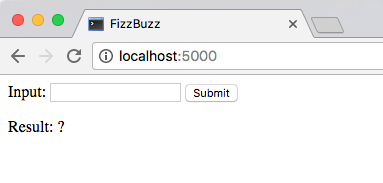
\includegraphics[width=4in]{figures/flask-web-server-local}
  \caption{Flask Web server on local machine.}
  \label{fig:flask-web-server-local}
\end{figure}

\noindent Let's see the code in {\tt app.py} under the {\tt web} folder.

\begin{verbatim}
from flask import Flask, render_template, request

from fizzbuzz import fizzbuzz


app = Flask(__name__)


@app.route('/', methods=['GET', 'POST'])
def index():
    result = '?'

    if request.method == 'POST':
        number = int(request.form.get('number'))
        result = fizzbuzz(number)

    return render_template('index.html', result=result)


if __name__ == '__main__':
    app.run(host='0.0.0.0', port=5000, debug=True)
\end{verbatim}

\noindent Play around with the application and take some minutes to understand
how the code works.

\subsection*{Getting Started with ATDD using Robot Framework}

\noindent Let's go back to the folder {\tt hello-robotframework} and open the
script {\tt fizzbuzz.robot} under the folder {\tt testcases}.

\begin{verbatim}
*** Settings ***
Resource         ../resources/common_res.txt
Test Setup       Go to homepage
Test Teardown    Close Browser


*** Variables ***
${HOMEPAGE}    http://localhost:5000/
${BROWSER}     chrome


*** Keywords ***
Go to homepage
    Open Browser    ${HOMEPAGE}    ${BROWSER}


*** Test Cases ***
Go to app and see the initial page
    Page Should Contain              Input:
    Page Should Contain              Result: ?
    Page Should Contain Textfield    name=number
    Page Should Contain Button       Submit

Go to app and input 3 then should see Fizz
    Input Text             name=number    3
    Submit Form
    Page Should Contain    Result: Fizz
\end{verbatim}

\noindent Here we already have two test cases. Let's try running it using the
command below:

\begin{verbatim}
$ robot testcases/fizzbuzz.robot
\end{verbatim}

\noindent See if the script works or not. If it does, let's take a minute to
understand the output before we move on. \\

\noindent {\bf Note:} Keep the FizzBuzz Web application up and running and use
the right virtual environment. \\

\noindent Now we want to continue developing the FizzBuzz program. We want it
to print ``Fizz'' out if the input is 6; therefore, we add a new test case.

\begin{verbatim}
Go to app and input 6 then should see Fizz
    Input Text             name=number    6
    Submit Form
    Page Should Contain    Result: Fizz
\end{verbatim}

\noindent Run the robot again. We should get the output like this:

\begin{verbatim}
==============================================================================
Fizzbuzz
==============================================================================
Go to app and see the initial page                                    | PASS |
------------------------------------------------------------------------------
Go to app and input 3 then should see Fizz                            | PASS |
------------------------------------------------------------------------------
Go to app and input 6 then should see Fizz                            | FAIL |
Page should have contained text 'Result: Fizz' but did not
------------------------------------------------------------------------------
Fizzbuzz                                                              | FAIL |
3 critical tests, 2 passed, 1 failed
3 tests total, 2 passed, 1 failed
==============================================================================
Output:  /Users/zkan/Projects/hello-robotframework/output.xml
Log:     /Users/zkan/Projects/hello-robotframework/log.html
Report:  /Users/zkan/Projects/hello-robotframework/report.html
\end{verbatim}

\noindent As seen in the output above, our new test case fails as expected. We
first create a new test case then we fix it by implementing that feature in the
actual code. This is the ATDD process. The feedback loop starts now.  Take your
time. :-) \\\\

\noindent ``Learning is experience. Everything else is just information.'' ---
Albert Einstein

\end{document}
